\documentclass[border=3pt]{standalone}
% Preâmbulo compartilhado pelos diagramas TikZ da aula 4 de Navegação (Representação de Mapas)
\usepackage[T1]{fontenc}
\usepackage[utf8]{inputenc}
\usepackage{lmodern}
\usepackage{amsmath}
\usepackage{xcolor}
\usepackage{tikz}
\usetikzlibrary{arrows.meta,angles,quotes,decorations.pathmorphing,decorations.pathreplacing,calc,
                positioning,shapes.geometric,shapes.misc,backgrounds,fit,
                math}

% Paleta (mesma dos SVGs originais)
\definecolor{dblue}{HTML}{2A5B8C}
\definecolor{dorange}{HTML}{B3541E}
\definecolor{dgreen}{HTML}{4A7C59}
\definecolor{dred}{HTML}{9C4B4B}
\definecolor{dcream}{HTML}{F4F1EA}
\definecolor{dshade}{HTML}{DDD7C9}

% Função gaussiana (não normalizada por padrão de escala visual)
\pgfmathdeclarefunction{gauss}{3}{%
  \pgfmathparse{1/(#3*sqrt(2*pi))*exp(-((#1-#2)^2)/(2*#3^2))}%
}

% Estilos comuns (prefixo d... para não colidir com chaves internas do pgf)
\tikzset{
  >={Stealth[length=2mm]},
  dguide/.style={gray!55, dashed, line width=0.4pt},
  daxis/.style={gray!60, line width=0.7pt, ->},
  dbody/.style={fill=black!3, draw=black!80, line width=1pt},
  dacc/.style={draw=dblue, line width=1pt},
  dlbl/.style={black!55, font=\small},
  dsub/.style={black!45, font=\footnotesize},
  dstate/.style={circle, draw=black!80, fill=dcream, line width=1pt,
                 minimum size=17mm, font=\large, inner sep=1pt},
  dobs/.style={circle, draw=black!80, fill=dshade, line width=1pt,
               minimum size=14mm, font=\large, inner sep=1pt},
  dbox/.style={rounded corners=2pt, draw=black!80, fill=dcream, line width=1pt,
               align=center, inner sep=6pt},
  dop/.style={circle, draw=black!80, fill=white, line width=1pt,
              minimum size=6mm, inner sep=0pt, font=\small},
  dtrans/.style={->, dblue, line width=1pt},
  dmeas/.style={->, dorange, line width=1pt},
  dcurve/.style={line width=1pt, dblue},
  dcurveb/.style={line width=1.4pt, dorange},
}

\begin{document}
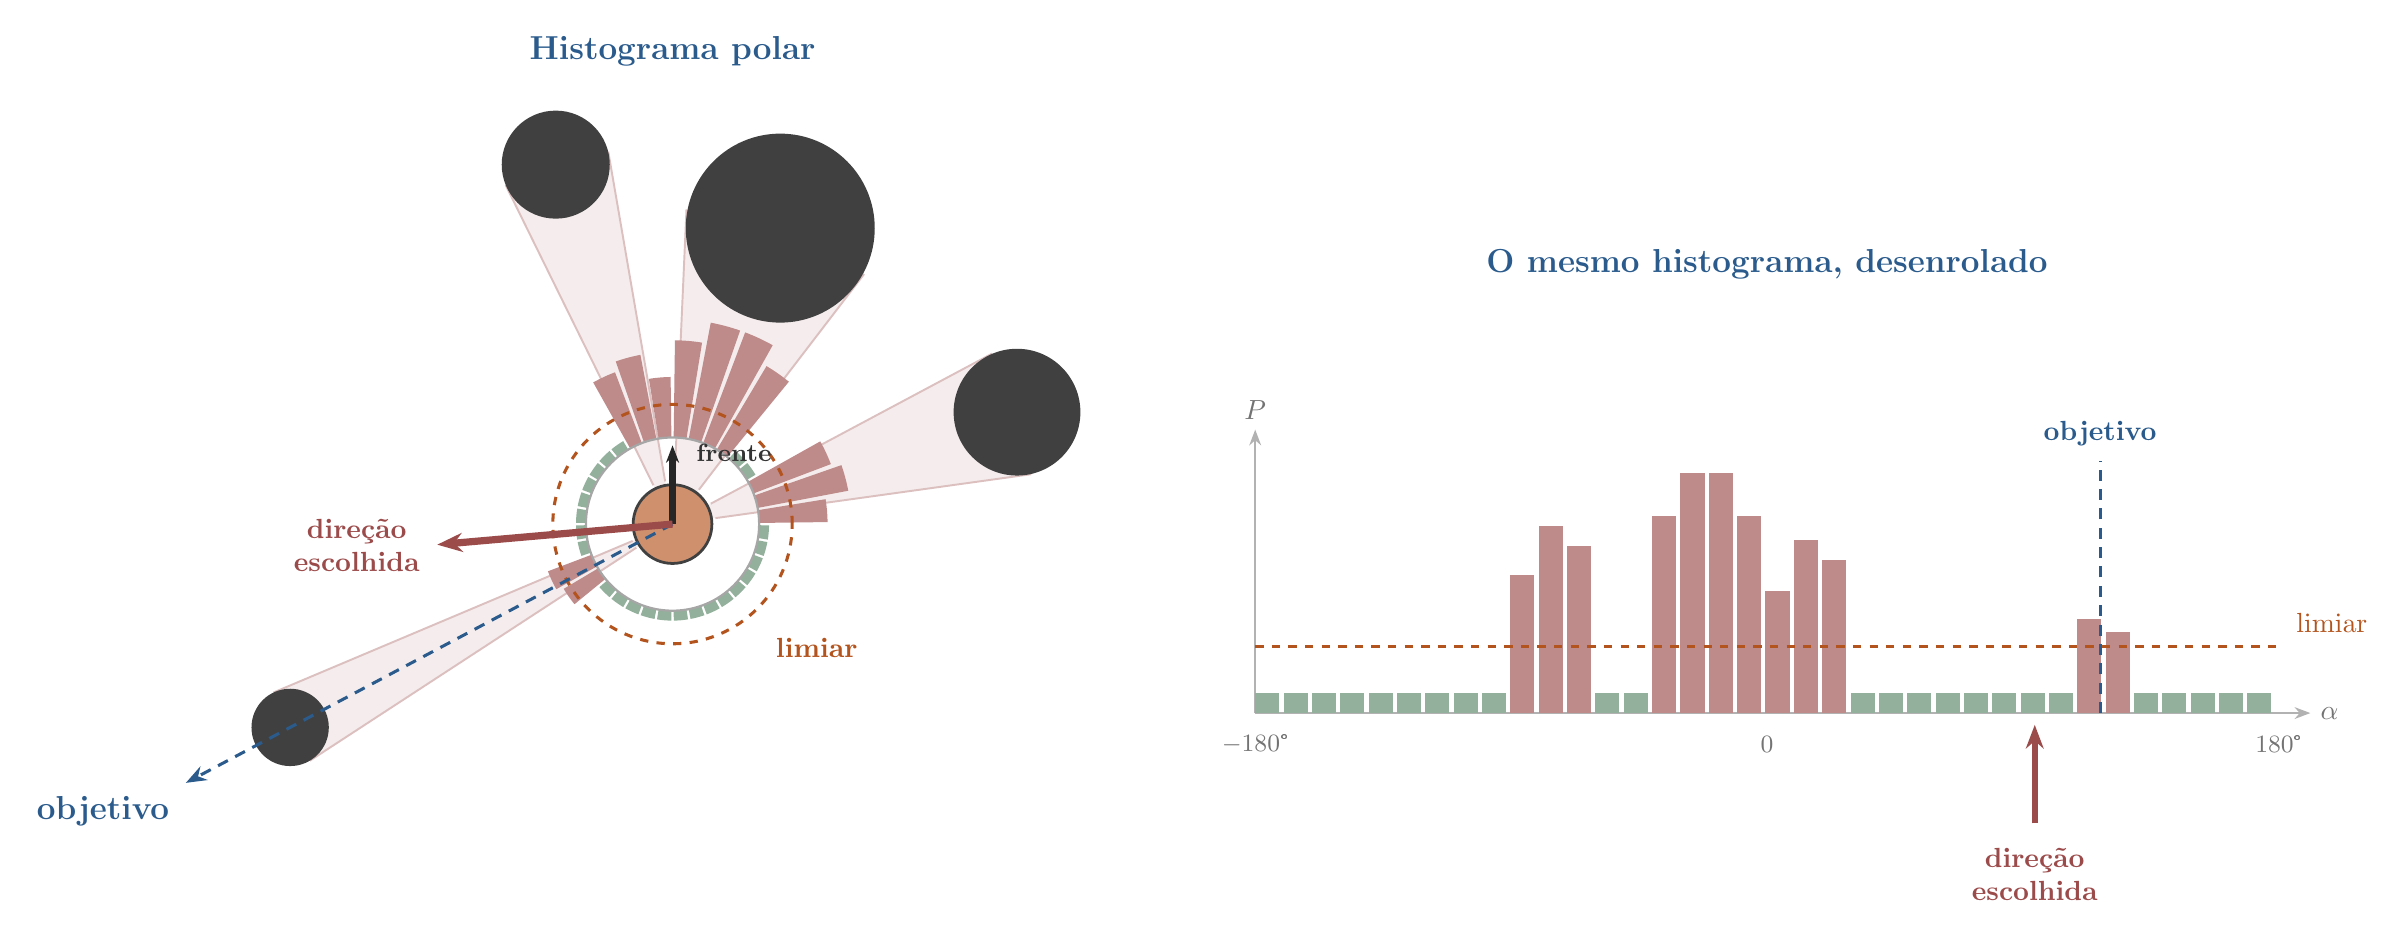
\begin{tikzpicture}[x=1cm,y=1cm]

  \def\heights{{
    0.3,0.3,0.3,0.3,0.3,0.3,
    0.3,0.3,0.3,2.07,2.79,2.5,
    0.3,0.3,2.94,3.58,3.58,2.94,
    1.83,2.59,2.29,0.3,0.3,0.3,
    0.3,0.3,0.3,0.3,0.3,1.41,
    1.21,0.3,0.3,0.3,0.3,0.3
  }}

  % ================= Painel polar =================
  \begin{scope}[shift={(5.6,5.6)}]
    \def\R{1.1}      % raio da base (valor zero)
    \def\k{0.42}     % escala radial
    \node[font=\bfseries\large, dblue] at (0,6.0) {Histograma polar};

    % cones de sombra dos obstáculos (mesmo ângulo das barras vermelhas)
    \fill[dred!10!white] (0,0) -- (52.54:4.00) arc (52.54:87.46:4.00) -- cycle;
    \draw[dred!35!white, line width=0.7pt] (52.54:0.55) -- (52.54:4.00) (87.46:0.55) -- (87.46:4.00);
    \fill[dred!10!white] (0,0) -- (7.92:4.60) arc (7.92:28.08:4.60) -- cycle;
    \draw[dred!35!white, line width=0.7pt] (7.92:0.55) -- (7.92:4.60) (28.08:0.55) -- (28.08:4.60);
    \fill[dred!10!white] (0,0) -- (99.79:4.80) arc (99.79:116.21:4.80) -- cycle;
    \draw[dred!35!white, line width=0.7pt] (99.79:0.55) -- (99.79:4.80) (116.21:0.55) -- (116.21:4.80);
    \fill[dred!10!white] (0,0) -- (202.88:5.50) arc (202.88:213.12:5.50) -- cycle;
    \draw[dred!35!white, line width=0.7pt] (202.88:0.55) -- (202.88:5.50) (213.12:0.55) -- (213.12:5.50);
    % setores (alpha = -180 + 10 i, medido a partir da frente do robô = para cima, anti-horário)
    \foreach \i in {0,...,35} {
      \pgfmathsetmacro{\h}{\heights[\i]}
      \pgfmathsetmacro{\a}{90-180+10*\i+0.75}
      \pgfmathsetmacro{\b}{90-180+10*\i+9.25}
      \pgfmathsetmacro{\ro}{\R+\k*\h}
      \ifdim\h pt>1.0pt
        \def\col{dred!65!white}
      \else
        \def\col{dgreen!60!white}
      \fi
      \fill[\col] (\a:\R) -- (\a:\ro) arc (\a:\b:\ro) -- (\b:\R) arc (\b:\a:\R) -- cycle;
    }
    \draw[black!35, line width=0.8pt] (0,0) circle (\R);
    \draw[dorange, dashed, line width=1.1pt] (0,0) circle (\R+\k*1.0);

    % obstáculos ao redor (onde a ocupação é alta)
    \fill[black!75] (70:4.00) circle (1.200);
    \fill[black!75] (18:4.60) circle (0.805);
    \fill[black!75] (108:4.80) circle (0.686);
    \fill[black!75] (208:5.50) circle (0.491);

    % robô, frente, objetivo e direção escolhida
    \fill[dorange!65, draw=black!75, line width=1pt] (0,0) circle (0.5);
    \draw[black!85, line width=2.4pt, -{Stealth[length=2.2mm]}] (0,0) -- (90:1.0);
    \node[font=\small\bfseries, black!80, anchor=west] at (0.18,0.9) {frente};
    \node[dorange, font=\normalsize\bfseries, anchor=north west, fill=white, inner sep=1pt] at (312:1.9) {limiar};
    \draw[dblue, line width=1.1pt, dash pattern=on 4pt off 3pt, -{Stealth[length=2.6mm]}] (0,0) -- (208:7.0);
    \node[dblue, font=\large\bfseries, anchor=north east] at (208:7.1) {objetivo};
    \draw[dred, line width=2.6pt, -{Stealth[length=3.2mm]}] (0,0) -- (185:3.0);
    \node[dred, font=\normalsize\bfseries, align=center, anchor=east] at (185:3.1) {direção\\escolhida};
  \end{scope}

  % ================= Painel linear =================
  \begin{scope}[shift={(13.0,3.2)}]
    \def\bw{0.36}
    \def\sc{0.85}
    \node[font=\bfseries\large, dblue] at (6.5,5.7) {O mesmo histograma, desenrolado};
    \draw[daxis] (0,0) -- (13.4,0) node[right, dlbl, font=\normalsize] {$\alpha$};
    \draw[daxis] (0,0) -- (0,3.6) node[above, dlbl, font=\normalsize] {$P$};
    \foreach \i in {0,...,35} {
      \pgfmathsetmacro{\h}{\heights[\i]}
      \ifdim\h pt>1.0pt
        \def\col{dred!65!white}
      \else
        \def\col{dgreen!60!white}
      \fi
      \fill[\col] (\i*\bw,0) rectangle ++(\bw*0.85,\sc*\h);
    }
    \draw[dorange, dashed, line width=1.1pt] (0,\sc*1.0) -- (13.0,\sc*1.0);
    \node[dorange, font=\normalsize, anchor=west] at (13.1,\sc*1.0+0.3) {limiar};
    \node[dlbl, font=\small] at (0,-0.4) {$-180${\textdegree}};
    \node[dlbl, font=\small] at (6.5,-0.4) {$0$};
    \node[dlbl, font=\small] at (13,-0.4) {$180${\textdegree}};
    % direção escolhida (alpha ~ 75°) e objetivo (alpha ~ 100°)
    \draw[dred, line width=2.2pt, -{Stealth[length=3mm]}] (9.9,-1.4) -- (9.9,-0.15);
    \node[dred, font=\normalsize\bfseries, align=center] at (9.9,-2.05) {direção\\escolhida};
    \draw[dblue, line width=1.1pt, dash pattern=on 4pt off 3pt] (10.73,0) -- (10.73,3.2);
    \node[dblue, font=\normalsize\bfseries] at (10.73,3.55) {objetivo};
  \end{scope}

\end{tikzpicture}
\end{document}
